\documentclass[a4paper]{article}

\usepackage[czech]{babel} %https://github.com/michal-h21/biblatex-iso690
\usepackage[
   backend=biber      % if we want unicode 
  ,style=iso-numeric % or iso-numeric for numeric citation method          
  ,babel=other        % to support multiple languages in bibliography
  ,sortlocale=cs_CZ   % locale of main language, it is for sorting
  ,bibencoding=UTF8   % this is necessary only if bibliography file is in different encoding than main document
]{biblatex}

\usepackage[utf8]{inputenc}
\usepackage{fancyhdr}
\usepackage{amsmath}
\usepackage{amssymb}
\usepackage[left=2cm,right=2cm,top=2.5cm,bottom=2.5cm]{geometry}
\usepackage{graphicx}
\usepackage{pdfpages}
\usepackage{url}

\usepackage{siunitx}
\sisetup{locale = DE}  %, separate-uncertainty = true    kdybych chtel +/-

\usepackage{float}
\newfloat{graph}{htbp}{grp}
\floatname{graph}{Graf}
\newfloat{tabulka}{htbp}{tbl}
\floatname{tabulka}{Tabulka}

\renewcommand{\thefootnote}{\roman{footnote}}

\pagestyle{fancy}
\lhead{Praktikum I - (XVI) Studium Brownova pohybu}
\rhead{Vladislav Wohlrath}
\author{Vladislav Wohlrath}

\bibliography{source}

\begin{document}

\begin{titlepage}
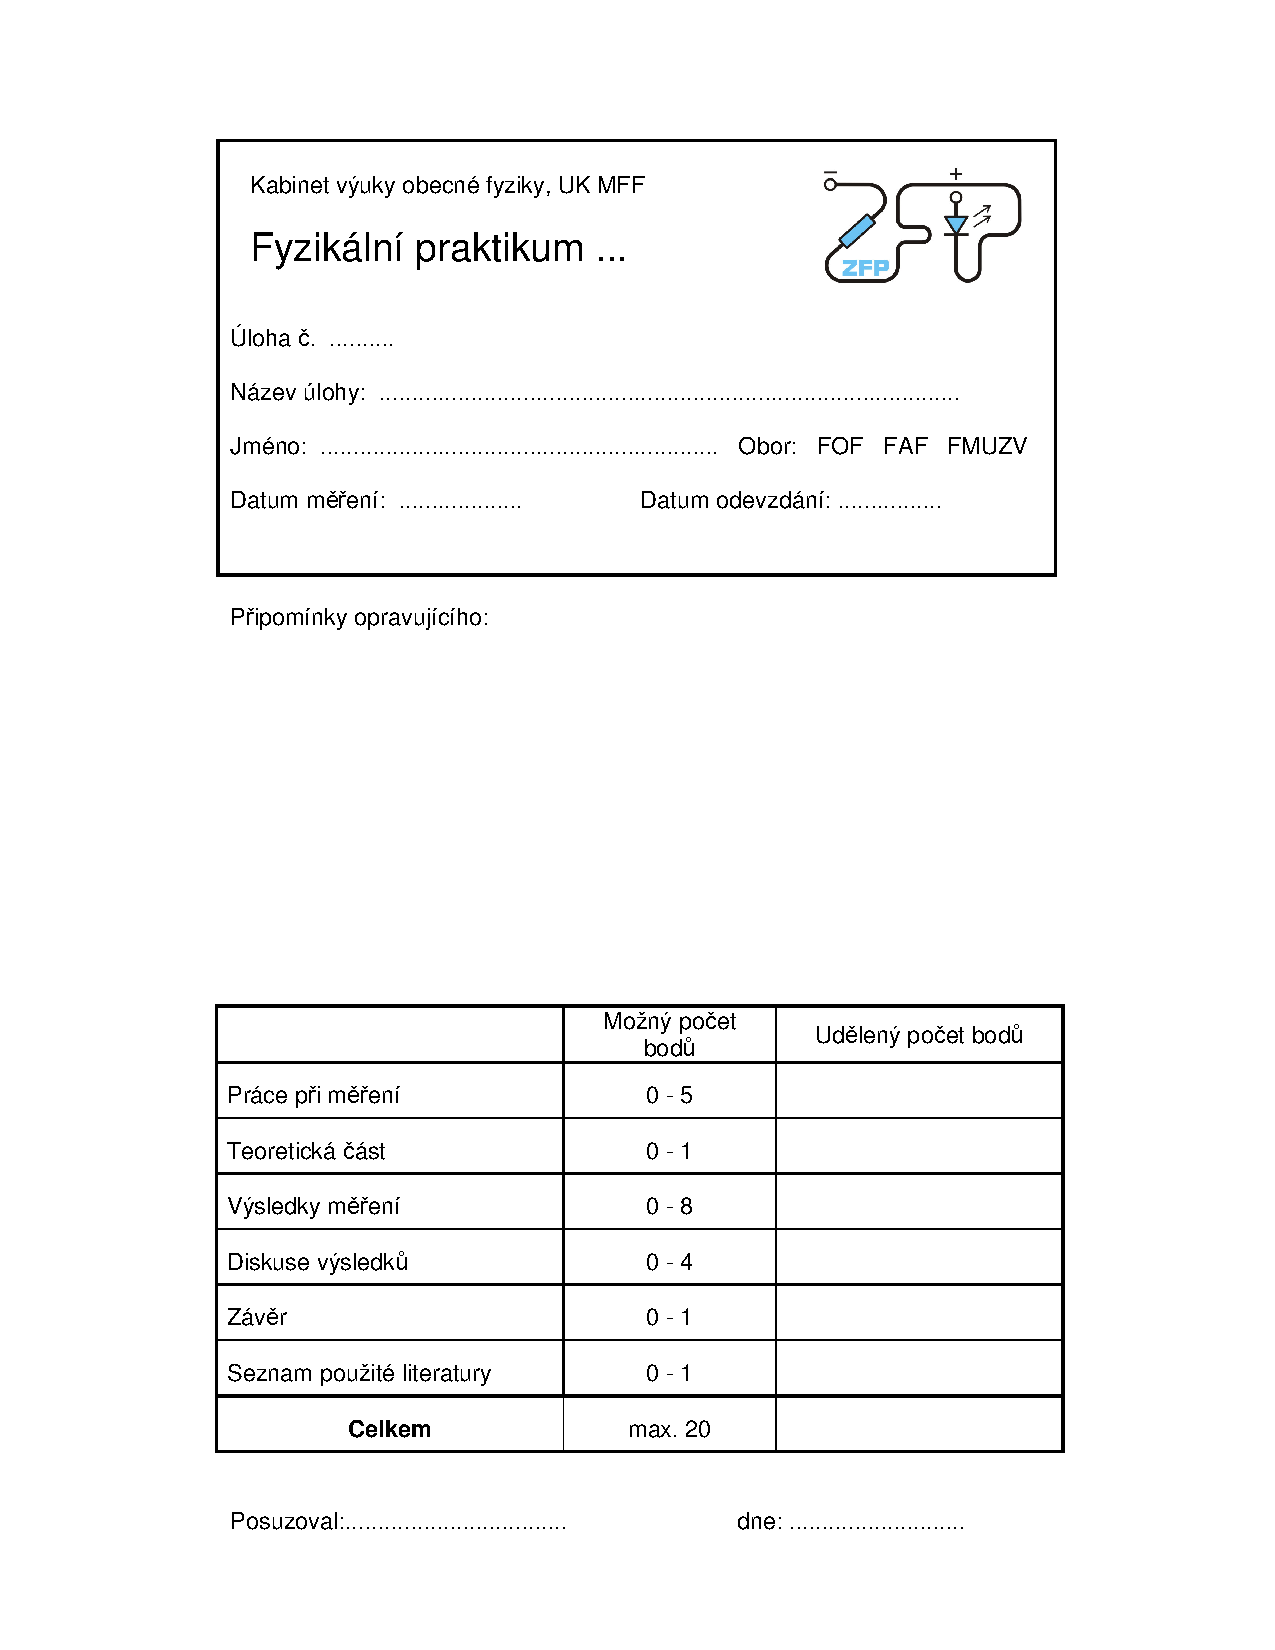
\includepdf[pages={1}]{./graficos/titlelist.pdf}
\end{titlepage}

\section*{Pracovní úkoly}
\begin{enumerate}
\item ÚKOLY
\end{enumerate}

%Teoretická část
\section*{Teoretická část}
Budeme mikroskpem pozorovat pohyb částic latexu ve vodě.
Pokud budeme zaznamenávat pouze průmět polohy částice do roviny, platí pro střední kvadratické posunutí $\overline{s^2}$ za čas $t$ vztah \cite{skripta}
\begin{equation} \label{eq::drahaaktivita}
\overline{s^2}=2 \cdot A \cdot t \,,
\end{equation}
kde $A$ je tzv. aktivita Brownova pohybu.
Pro kulové částice o poloměru $r$ v prostředí s teplotou $T$ a dynamickou viskozitou $\eta$ platí \cite{skripta}
\begin{equation} \label{eq::aktivitavzorec}
A=\frac{RT}{3 \pi \eta r N_A} \,,
\end{equation}
kde $R=~\SI{8.314}{\joule \per \mole \per \kelvin}$ je molární plynová konstanta a $N_A$ je Avogadrova konstanta.

Ze vztahu \eqref{eq::drahaaktivita} je zřejmé, že když budeme zaznamenávat dráhy částic za čas $t$, $2t$, $3t$ a $4t$ bude pro $s_t$, $s_{2t}$, $s_{3t}$ a $s_{4t}$ platit
\begin{equation}
\overline{s_t^2}:\overline{s_{2t}^2}:\overline{s_{3t}^2}:\overline{s_{4t}^2} = 1:2:3:4 \,.
\end{equation}

Pokud naměřená data budou splňovat tuto podmínku, použijeme naměřené střední kvadratické posunutí $\overline{s_t^2}$ k výpočtu aktivity $A$ a následně Avogadrovy konstanty $N_A$ úpravou vztahu \eqref{eq::aktivitavzorec}
\begin{equation}
A=\frac{\overline{s^2}}{2 \cdot t}
\end{equation}
\begin{equation}
N_A=\frac{2RTt}{3\pi \eta r \overline{s^2}}
\end{equation}
a odchylku metodou přenosu chyb
\begin{equation}
\sigma_A = A \sqrt{
\left( \frac{\sigma_{\overline{s^2}}}{\overline{s^2}}  \right)^2 +
\left( \frac{\sigma_t}{t}    \right)^2
}
\end{equation}
\begin{equation}
\sigma_{N_A}=N_A \sqrt{
\left( \frac{\sigma_T}{T} \right)^2  +
\left( \frac{\sigma_t}{t} \right)^2  +
\left( \frac{\sigma_\eta}{\eta} \right)^2  +
\left( \frac{\sigma_r}{r} \right)^2  +
\left( \frac{\sigma_{\overline{s^2}}}{\overline{s^2}} \right)^2
} \,.
\end{equation}

%Podmínky a měřící přístroje
\section*{Podmínky a použité přístroje}

%Výsledky měření
\section*{Výsledky měření}
Teplota vzorku byla $T =~\SI{0}{\kelvin}$.

Dynamickou viskozitu vody při této teplotě uvádí \cite{viskozita} $\eta=~\SI{0}{\m\square\per\s}$.

Poloměr částic latexu jsme určili podle fotografie z elektronového mikroskopu (viz příloha 1).
Změřili jsme poloměr \num{0} částic

Polohu částic jsme zaznamenávali v pravidelných časových intervalech $t=~\SI{0}{\s}$.



%Diskuze výsledků
\section*{Diskuze}
Částice v substrátu se nepohybovaly jen v pozorovací rovině, takže bylo nutno na ně během jejich pohybu zaostřovat.
Bohužel mikroskop se viklal a při zaostřování se obraz posouval.
Tato závada byla objevena až po čtvrtém měření, takže přiložené měření č. 1 a 3 jsou touto chybou ještě postiženy, což mělo pravděpodobně za následek jejich nepřílišnou shodu s \eqref{eq::pomerdrah1234}.
Poté jsme zvětšili hloubku ostrosti mikroskopu, aby se během pozorování pohybu částice nemuselo zaostřovat.

Při měřeních, které nejsou přiloženy, bylo zaznamenáno příliš málo poloh (méně než 50), vyskytl se preferovaný směr tečení, nebo jsme pozorovali shluk částic (střední kvadratická dráha byla výrazně menší než u měření č. 1, 3, 8).

Tabelovaná hodnota Avogadrovy konstanty \cite{avogadro} je $\num{6.022}\times 10^{23}\,\si{\per\mole}$.
Námi naměřená hodnota se od této hodnoty liší o \SI{31}{\percent}.
Shodu považujeme za dostatečnou vzhledem k velmi vysoké nepřesnosti naší metody.

%Závěr
\section*{Závěr}
Pozorovali jsme Brownův pohyb částic latexu ve vodě.
Ověřili jsme Einsteinův vztah pro střední kvadratické posunutí v čase, při měření č. 8 jsme naměřili za časy $t$, $2t$, $3t$ a $4t$ poměr středních kvadratických posunutí $1:\num[separate-uncertainty=false]{2.06(27)}:\num[separate-uncertainty=false]{3.09(40)}:\num[separate-uncertainty=false]{4.24(54)}$.
V závorkách jsou uvedeny standardní odchylky průměru v posledním uvedeném řádu.
Při ostatních měřeních nebyly výsledky přesvědčivé.

Střední kvadratické posunutí za čas $t=\SI{4.8}{\s}$ při měření č. 8 bylo \SI{18(2)}{\micro\metre\squared}.

Aktivita Brownova pohybu částic latexu ve vodě za pokojové teploty je \SI{1.87(21)}{\micro\metre\squared\per\s}.

Z aktivity Brownova pohybu jsme určili Avogadrovu konstantu $N_A = (7,9 \pm 1,3) \times 10^{23} \,\si{\per\mole}$. 
Tabelovaná hodnota \cite{avogadro} je $\num{6.022}\times 10^{23}\,\si{\per\mole}$. Naše hodnota se s ní v rámci jedné směrodatné odchylky sice neshoduje, nicméně řád jsme určili přesně.


\printbibliography[title={Seznam použité literatury}]

\end{document}